\begin{enumerate}
	\item Exercício
	
	Faça o esboço do sólido cujo volume é dado pela integral abaixo.
	
	\begin{equation*}
		v = \int_{-1}^1 \int_{-\sqrt{1 - x^2}}^{\sqrt{1 - x^2}} \int_0^{y + 1} dzdydx = \int_{-1}^1 dx \int_{-\sqrt{1 - x^2}}^{\sqrt{1 - x^2}} dy \int_0^{y + 1} dz
	\end{equation*}
	
	\begin{figure}[htb]
		\caption{Integrais triplas - Aula 04 - Exercício I}
		\label{v17_a04_e01}
		\centering
		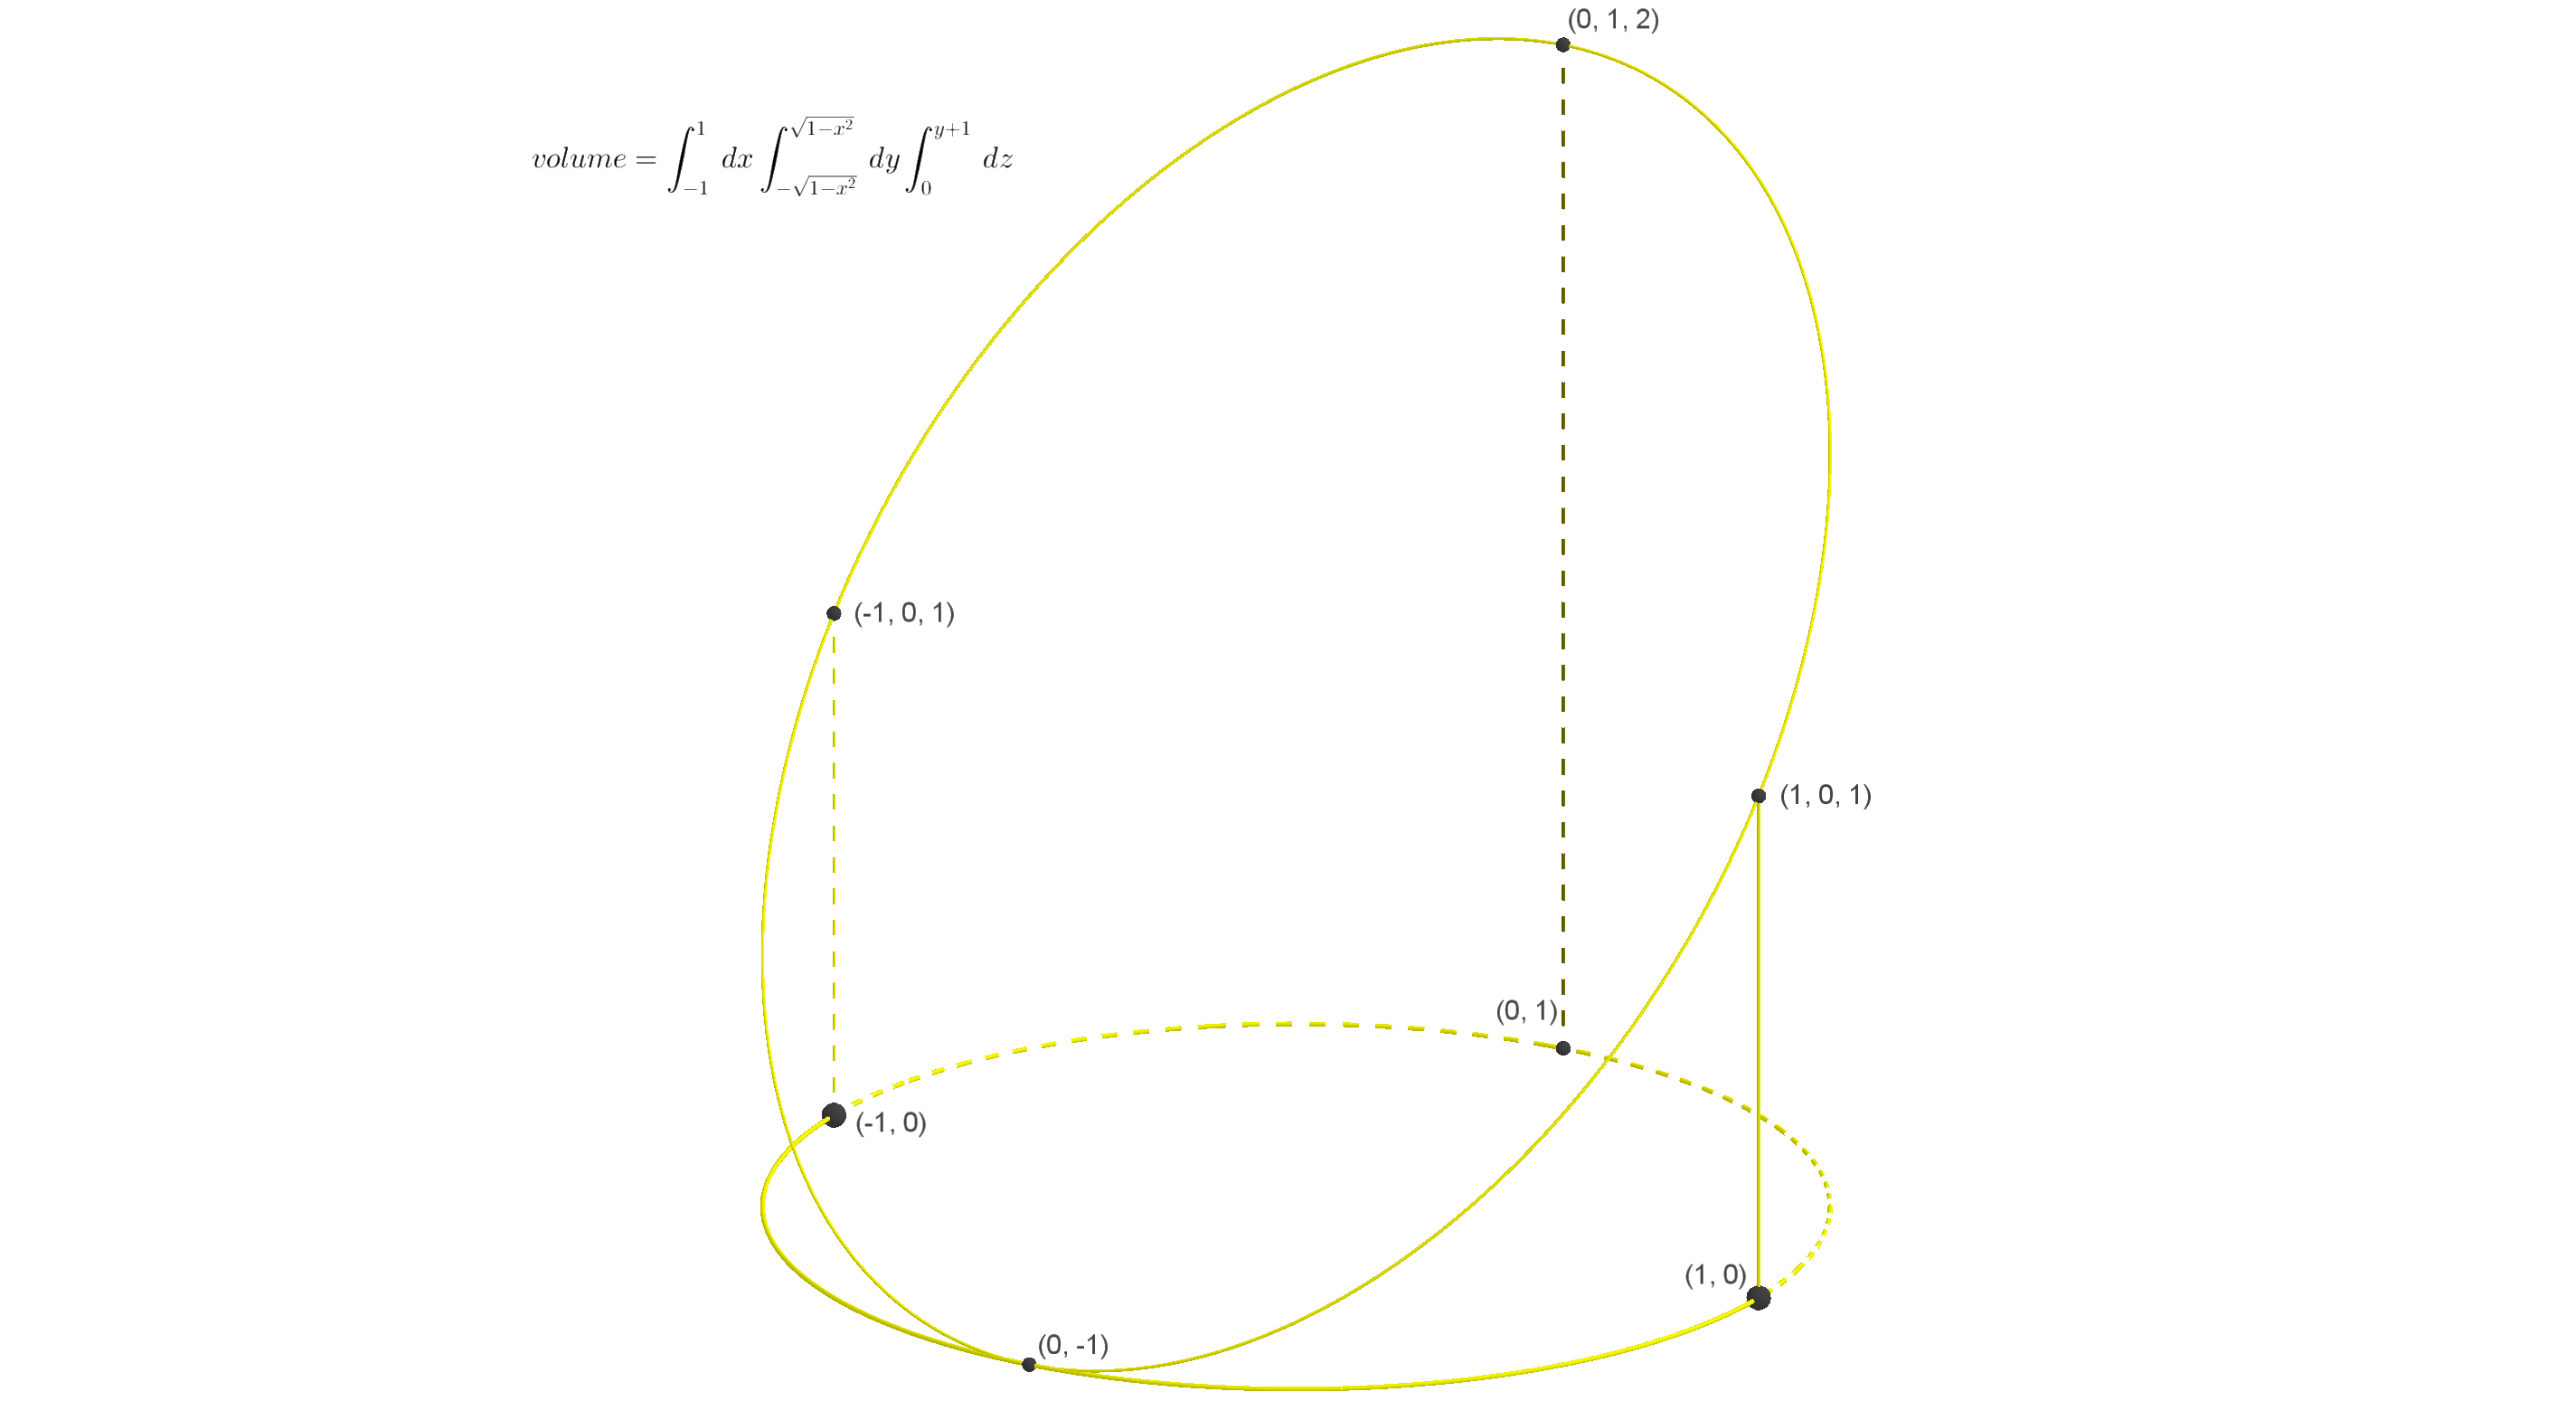
\includegraphics[width=0.5\textwidth]{v17_a04_e01.png}		
	\end{figure}
	
	\begin{align*}
		v = \int_{-1}^1 dx \int_{-\sqrt{1 - x^2}}^{\sqrt{1 - x^2}} dy \int_0^{y + 1} dz = \int_{-1}^1 dx \int_{-\sqrt{1 - x^2}}^{\sqrt{1 - x^2}} dy \left[z\right]_0^{y + 1} = \int_{-1}^1 dx \int_{-\sqrt{1 - x^2}}^{\sqrt{1 - x^2}} (y + 1)\, dy =\\ \int_{-1}^1 dx \left[\dfrac{y^2}{2} + y\right]_{-\sqrt{1 - x^2}}^{\sqrt{1 - x^2}} =\\ \int_{-1}^1 \left[\dfrac{\left(\sqrt{1 - x^2}\right)^2}{2} + \sqrt{1 - x^2} - \left(\dfrac{\left(-\sqrt{1 - x^2}\right)^2}{2} - \sqrt{1 - x^2}\right)\right] dx =\\ \int_{-1}^1 \left(\dfrac{1 - x^2}{2} + \sqrt{1 - x^2} - \dfrac{\left(1 - x^2\right)}{2} + \sqrt{1 - x^2}\right) dx =\\ \int_{-1}^1 \left(\dfrac{\overstrike{1}}{\overstrike{2}} - \dfrac{\overstrike{x^2}}{\overstrike{2}} + \sqrt{1 - x^2} - \dfrac{\overstrike{1}}{\overstrike{2}} + \dfrac{\overstrike{x^2}}{\overstrike{2}} + \sqrt{1 - x^2}\right) dx = \int_{-1}^1 \left(2\sqrt{1 - x^2}\right) dx =\\ 2\int_{-1}^1 \sqrt{1 - \sen^2(\theta)} \cos(\theta)\, d\theta = 2\int_{-1}^1 \sqrt{1 - \left(1 - \cos^2(\theta)\right)} \cos(\theta)\, d\theta =\\ 2\int_{-1}^1 \sqrt{ \cos^2(\theta)} \cos(\theta)\, d\theta = 2\int_{-1}^1 \cos^2(\theta)\, d\theta =  2\int_{-1}^1 \left(\dfrac{1 + \cos(2\theta)}{2}\right)\, d\theta =\\ 2\int_{-1}^1 \left(\dfrac{1}{2} + \dfrac{\cos(2\theta)}{2}\right)\, d\theta = \int_{-1}^1 d\theta + \int_{-1}^1 \cos(2\theta)\, d\theta = \int_{-1}^1 d\theta + \int_{-1}^1 \cos(u)\dfrac{du}{2} =\\ \int_{-1}^1 d\theta + \dfrac{1}{2}\int_{-1}^1 \cos(u)\, du = \left[\theta + \dfrac{\sen(u)}{2}\right]_{-1}^1 = \left[\theta + \dfrac{\sen(2\theta)}{2}\right]_{-1}^1 =\\ \left[\theta + \dfrac{\overstrike{2}\sen(\theta)\cos(\theta)}{\overstrike{2}}\right]_{-1}^1 = \left[\theta + \sen(\theta)\cos(\theta)\right]_{-1}^1 = \left[\arcsen(x) + x\sqrt{1 - x^2}\right]_{-1}^1 =\\ \left[\arcsen(1) \overstrike{+ 1\sqrt{1 - 1^2}} - \left(\arcsen(-1) \overstrike{+ (-1)\sqrt{1 - (-1)^2}}\right)\right] = \left[\arcsen(1) - \arcsen(-1)\right] =\\ \dfrac{\pi}{2} + \dfrac{\pi}{2} = \dfrac{\pi + \pi}{2} = \dfrac{2\pi}{2} = \pi
	\end{align*}
	\begin{equation*}
		x = \sen(\theta) \Rightarrow dx = \cos(\theta)\, d\theta
	\end{equation*}
	\begin{equation*}
		u = 2\theta \Rightarrow \dfrac{du}{2} = d\theta
	\end{equation*}
	\begin{equation*}
		\sen(\theta) = \dfrac{co}{h} = \dfrac{x}{1} = x;\; \theta = \arcsen(x)	
	\end{equation*}
	\begin{equation*}
		1 = x^2 + ca \Rightarrow ca = \sqrt{1 - x^2}
	\end{equation*}
	\begin{equation*}
		\cos(\theta) = \dfrac{ca}{h} = \dfrac{\sqrt{1 - x^2}}{1} = \sqrt{1 - x^2}
	\end{equation*}
	
	\item Exercício
	
	Faça o esboço do sólido cujo volume é dado pela integral abaixo.
	
	\begin{equation*}
		v = \int_0^1 \int_0^{\sqrt{1 - x^2}} \int_0^2 dydzdx = \int_0^1 dx \int_0^{\sqrt{1 - x^2}} dz \int_0^2 dy
	\end{equation*}
	
	\begin{figure}[htb]
		\caption{Integrais triplas - Aula 04 - Exercício II}
		\label{v17_a04_e02}
		\centering
		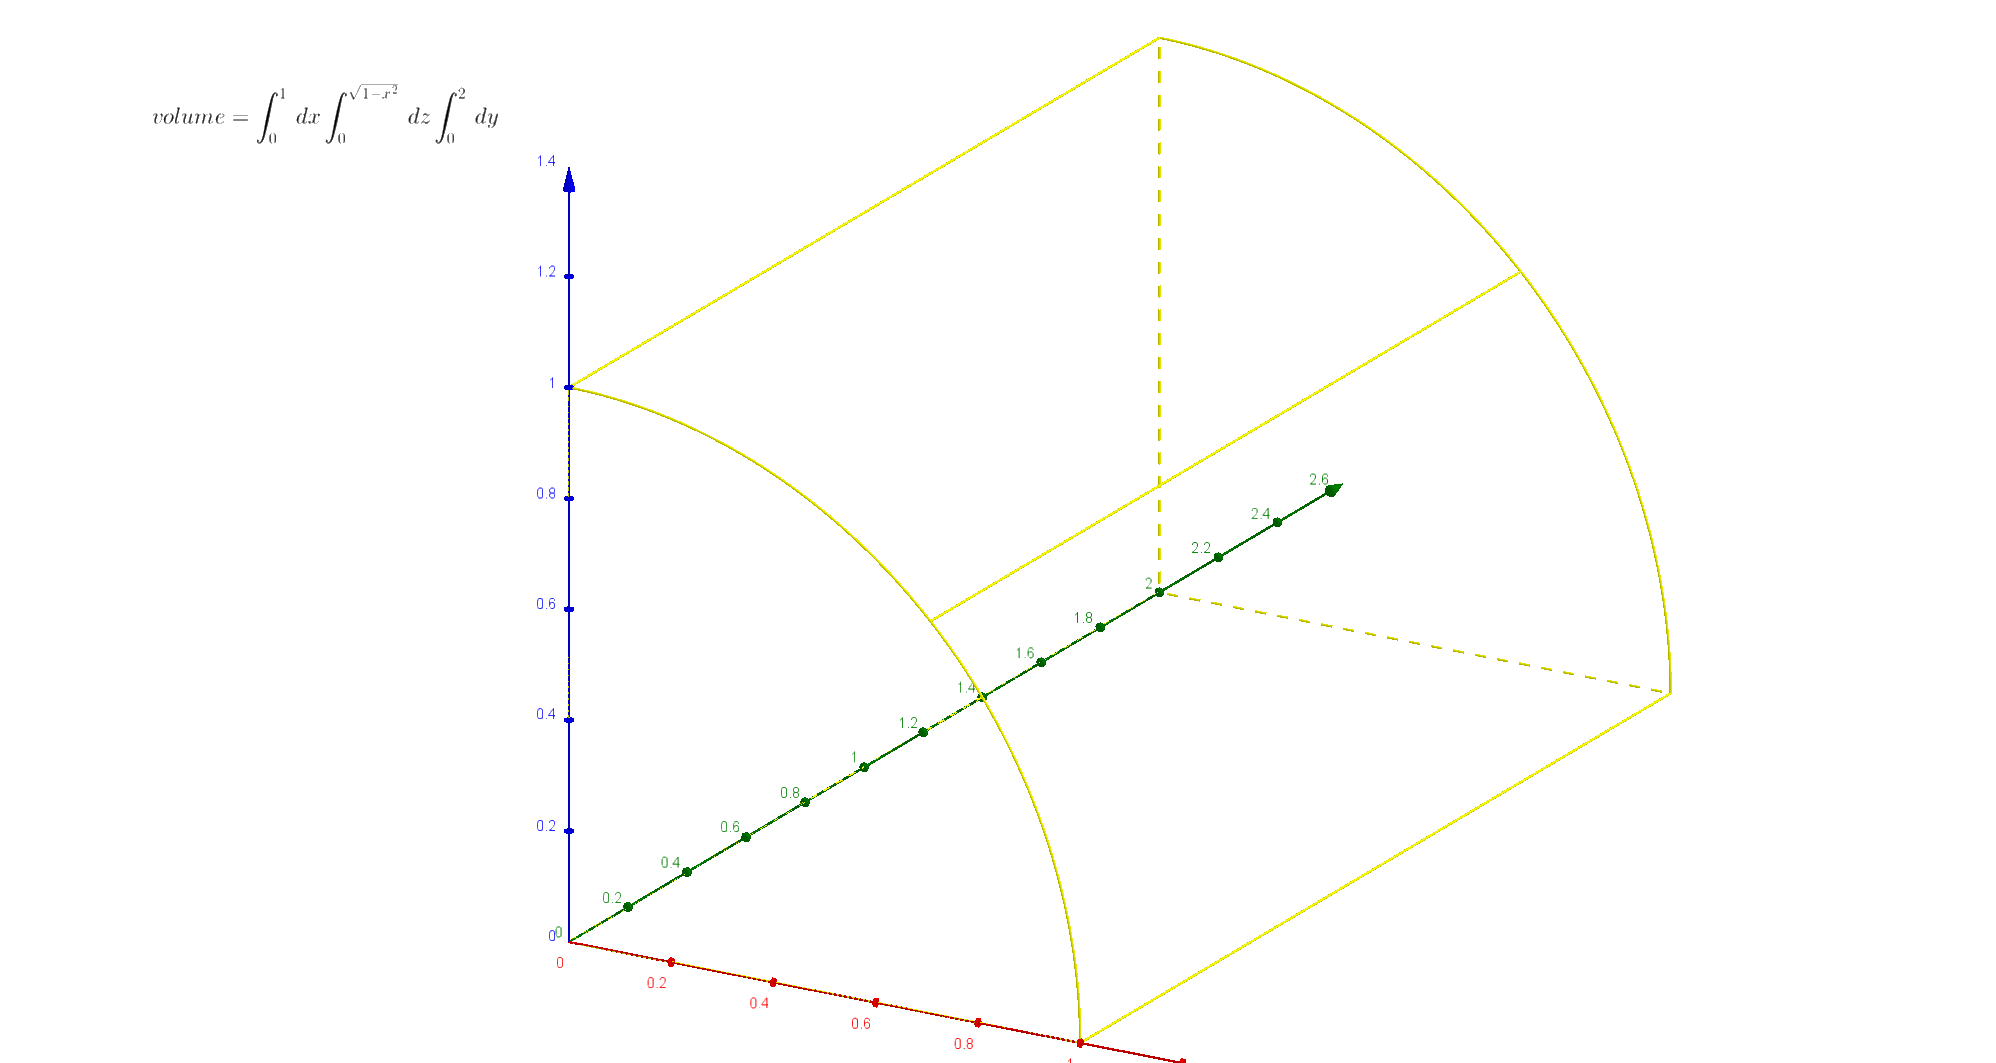
\includegraphics[width=0.5\textwidth]{v17_a04_e02.png}		
	\end{figure}
		
	\begin{align*}
		v = \int_0^1 dx \int_0^{\sqrt{1 - x^2}} dz \left[y\right]_0^2 = 2\int_0^1 dx \int_0^{\sqrt{1 - x^2}} dz = 2\int_0^1 dx \left[z\right]_0^{\sqrt{1 - x^2}} = 2\int_0^1 \sqrt{1 - x^2}\, dx =\\ 2\int_0^1 \sqrt{1 - \sen^2(\theta)}\cos(\theta)\, d\theta = 2\int_0^1 \sqrt{1 - \left(1 - \cos^2(\theta)\right)}\cos(\theta)\, d\theta =\\ 2\int_0^1 \sqrt{\cos^2(\theta)}\cos(\theta)\, d\theta = 2\int_0^1 \cos^2(\theta)\, d\theta = 2\int_0^1 \left(\dfrac{1 + \cos(2\theta)}{2}\right) d\theta =\\ 2\int_0^1 \left(\dfrac{1}{2} + \dfrac{\cos(2\theta)}{2}\right) d\theta = \int_0^1 d\theta + \int_0^1 \cos(2\theta)\, d\theta = \int_0^1 d\theta + \int_0^1 \cos(u)\dfrac{du}{2} =\\ \int_0^1 d\theta + \dfrac{1}{2}\int_0^1 \cos(u)\, du = \left[\theta + \dfrac{\sen(u)}{2}\right]_0^1  = \left[\theta + \dfrac{\sen(2\theta)}{2}\right]_0^1 = \left[\theta + \dfrac{\overstrike{2}\sen(\theta)\cos(\theta)}{\overstrike{2}}\right]_0^1 =\\ \left[\theta + \sen(\theta)\cos(\theta)\right]_0^1 = \left[\arcsen(x) + x\sqrt{1 - x^2}\right]_0^1 =\\ \arcsen(1) \overstrike{+ 1\sqrt{1 - 1^2}} - \left(\arcsen(0) \overstrike{+ 0\sqrt{1 - 0^2}}\right) = \arcsen(1) \overstrike{- \arcsen(0)} = \dfrac{\pi}{2}	
	\end{align*}
	\begin{equation*}
		x = \sen(\theta) \Rightarrow dx = \cos(\theta)\, d\theta
	\end{equation*}
	\begin{equation*}
		u = 2\theta \Rightarrow \dfrac{du}{2} = d\theta
	\end{equation*}
	\begin{equation*}
		\sen(\theta) = \dfrac{co}{h} = \dfrac{x}{1} = x;\; \theta = \arcsen(x)	
	\end{equation*}
	\begin{equation*}
		1 = x^2 + ca \Rightarrow ca = \sqrt{1 - x^2}
	\end{equation*}
	\begin{equation*}
		\cos(\theta) = \dfrac{ca}{h} = \dfrac{\sqrt{1 - x^2}}{1} = \sqrt{1 - x^2}
	\end{equation*}
	
	\item Exercício
	
	Faça o esboço do sólido cujo volume é dado pela integral abaixo.
	
	\begin{equation*}
		v = \int_{-1}^0 \int_0^1 \int_0^{y^2} dzdxdy = \int_{-1}^0 dy \int_0^1 dx \int_0^{y^2} dz	
	\end{equation*}
	
	\begin{figure}[htb]
		\caption{Integrais triplas - Aula 04 - Exercício III}
		\label{v17_a04_e03}
		\centering
		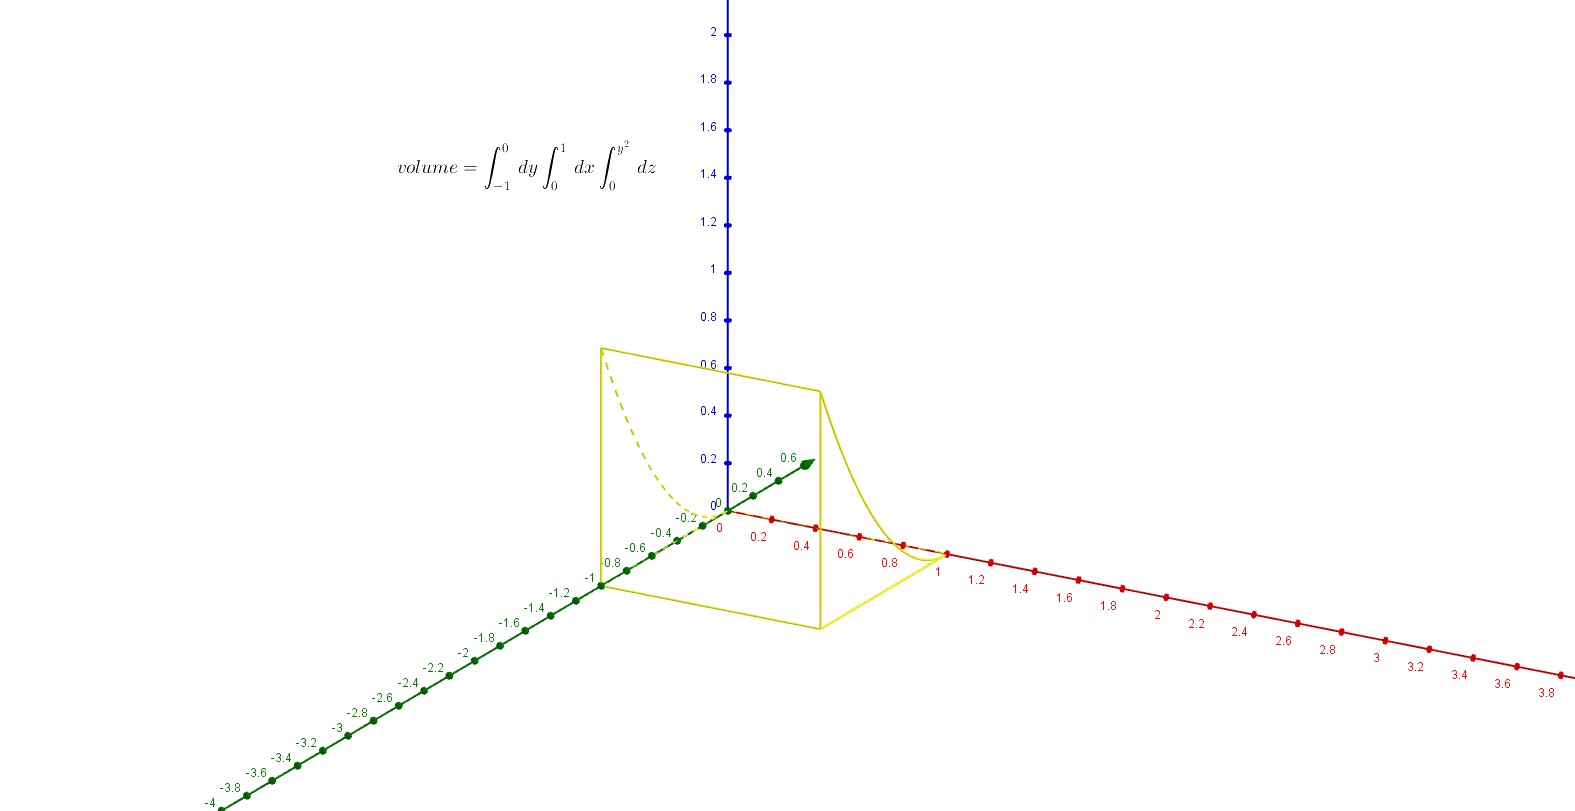
\includegraphics[width=0.5\textwidth]{v17_a04_e03.png}		
	\end{figure}
	
	\begin{align*}
		v = \int_{-1}^0 dy \int_0^1 dx \int_0^{y^2} dz = \int_{-1}^0 dy \int_0^1 dx \left[z\right]_0^{y^2} = \int_{-1}^0 y^2 dy \int_0^1 dx = \int_{-1}^0 y^2 dy \left[x\right]_0^1 =\\ \int_{-1}^0 y^2 dy = \left[\dfrac{y^3}{3}\right]_{-1}^0 = \dfrac{\overstrike{0^3}}{\overstrike{3}} - \dfrac{(-1)^3}{3} = \dfrac{1}{3}
	\end{align*}
\end{enumerate}